\documentclass[journal,twoside,web]{ieeecolor}
\usepackage{tmi}
\usepackage{booktabs}
\usepackage{cite}
\usepackage{amsmath,amssymb,amsfonts}
\usepackage{algorithm}
\usepackage{algpseudocode}
\usepackage{graphicx}
\usepackage{siunitx}
\usepackage{textcomp}

\usepackage{color,soul}
\usepackage{xcolor}

\makeatletter
\let\NAT@parse\undefined
\makeatother
\usepackage{hyperref}

\usepackage[capitalise,noabbrev]{cleveref}


\def\BibTeX{{\rm B\kern-.05em{\sc i\kern-.025em b}\kern-.08em
	T\kern-.1667em\lower.7ex\hbox{E}\kern-.125emX}}
\markboth{\journalname, VOL. XX, NO. XX, XXXX 2024}
{Tan \MakeLowercase{\textit{et al.}}: Self-Gated ADMM Unrolling for High-Resolution DWI}


\newcommand{\argmin}{\operatornamewithlimits{argmin}}
\newcommand{\norm}[1]{\left\lVert#1\right\rVert}


% FK:
% 1. start with problem statement
% 2. current solution and limitation
%
% Blackbox is not in favor

\begin{document}
	\title{High-Resolution Motion-Robust Diffusion-Weighted Imaging with Self-Gated  Self-Supervised ADMM Unrolling}

	\author{Zhengguo Tan, Patrick A Liebig, Annika Hofmann, Frederik B Laun, Florian Knoll
		\thanks{This work was supported in part by
			German Research Foundation (DFG)
			under projects 513220538 and 512819079,
			project 500888779 in the Research Unit RU5534
			for MR biosignatures at UHF,
			and by the National Institutes of Health (NIH)
			under grants R01EB024532 and P41EB017183.
			In addition, scientific support and HPC resources
			were provided by
			the Erlangen National High Performance Computing Center (NHR)
			of Friedrich-Alexander-University Erlangen-Nuremberg (FAU)
			under the NHR project b143dc.
			NHR is funded by federal and Bavarian state authorities.
			NHR@FAU hardware is partially funded by
			DFG under project 440719683. \textit{(Corresponding Author:~Zhengguo Tan)}}
		\thanks{Z.~Tan was with the Department
			Artificial Intelligence in Biomedical Engineering (AIBE),
			FAU, Erlangen, Germany.
			He is now with
			the Michigan Institute for Imaging Technology and Translation
			(MIITT),
			Department of Radiology,
			University of Michigan, Ann Arbor, MI 48109 USA
			(e-mail: zgtan@med.umich.edu).}
%		\thanks{J.~Glaser was with the Department of Medical Engineering,
%			FAU, Erlangen, Germany.
%			He is now with the Institute of Radiology,
%			University Hospital Erlangen,
%			FAU, Erlangen, Germany
%			(e-mail: julius.glaser@fau.de).}
		\thanks{P.~A.~Liebig is with Siemens Healthcare GmbH, Erlangen, Germany
			(e-mail: patrick.liebig@siemens-healthineers.com).}
		\thanks{A.~Hofmann is with the Department AIBE,
			FAU, Erlangen, Germany
			(e-mail: annika.ah.hofmann@fau.de).}
		\thanks{F.~B.~Laun is with the Institute of Radiology,
			University Hospital Erlangen,
			FAU, Erlangen, Germany
			(e-mail: Frederik.Laun@uk-erlangen.de).}
		\thanks{F.~Knoll is with the Department AIBE,
			FAU, Erlangen, Germany
			(e-mail: florian.knoll@fau.de).}
	}

	\maketitle

	% Keep the abstract to 250 words or less.
	\begin{abstract}
		This work introduces a self-gated self-supervised learning joint reconstruction framework for navigator-free, high-resolution, and motion-robust diffusion-weighted imaging (DWI) based on undersampled multi-shot interleaved echo-planar imaging (iEPI) acquisition. Specifically, the proposed self-supervised learning unrolls the alternating direction method of multipliers (ADMM). The ADMM unrolling alternatively minimizes a physics-guided data-consistency term and a learned regularization function. Two-dimensional residual neural network (ResNet) is employed as the learnable regularization to leverage redundancy in the spatial-diffusion dimension.
		First, we perform a computational experiment in which ADMM unrolling is trained with only one multi-band slice out of the volumetric brain DWI acquisition, and the trained model is then inferred on all remaining slices. This experiment demonstrates the model's cross-slice generalization feature, where the trained model is applicable to "unseen" slices.
		Second, the proposed self-gated ADMM unrolling is validated with both retrospectively and prospectively acquired data at 0.7 mm isotropic resolution. Our method outperforms both multiplexed sensitivity-encoding (MUSE) and compressed sensing with locally-low rank (LLR) regularization in terms of image sharpness, tissue continuity and motion robustness.
		Third, ADMM unrolling converges sufficiently in 100 epochs, 
		and enables the learning of the regularization strength.
		Fourth, although ADMM unrolling requires up to eight hours training per slice, its inference time is just one minute. In comparison, LLR requires about an hour per slice.
		Overall, self-gated self-supervised ADMM unrolling enables undersampled multi-shot iEPI acquisition without the need of navigators, providing sub-millimeter DWI at clinically feasible reconstruction times. The source code is publicly available at:~\url{https://github.com/ZhengguoTan/DeepDWI}.
	\end{abstract}

	\begin{IEEEkeywords}
	Magnetic resonance imaging, MR physics, Diffusion weighted imaging, Image reconstruction, Machine learning, End-to-end learning in medical imaging, Inverse methods, Optimization, Image acquisition
	\end{IEEEkeywords}

	% ============================== %
	\section{Introduction}
	\label{SEC:INTRO}
	\IEEEPARstart{H}{igh}-dimensional magnetic resonance imaging (HD-MRI)
	has been a flourishing field,
	focused on the acquisition, reconstruction and analysis of
	multi-dimensional multi-contrast-weighted MRI data.
	Examples of HD-MRI include but are not limited to
	magnetic resonance spectroscopic imaging (MRSI)
	\cite{brown_1982_mrsi},
	diffusion-weighted imaging (DWI)
	\cite{jones_2010_diff},
	and quantitative parameter mapping
	\cite{doneva_2010_moba,ma_2013_mrf}.
	Conventional HD-MRI, however, requires long acquisition times,
	making the data susceptible to subject motion
	and system imperfections, and imposing high computational burden.
	DWI, in particular, poses challenges in the pursuit of
	high spatial, temporal, and angular resolution.
	DWI is typically acquired using
	the pulsed gradient spin echo diffusion-weighted sequence 
	\cite{stejskal_1965_pgse}
	followed by fast echo-planar imaging (EPI) readouts
	\cite{mansfield_1977_epi}.
	However, the use of long echo trains in EPI results in
	geometric distortion artifacts and reduced spatial resolution.
	Additionally, acquiring multiple diffusion directions
	to enhance angular resolution and
	to better probe tissue microstructure further extends the scan time.

	Advances in parallel imaging
	\cite{roemer_1990_pi,sodickson_1997_smash,
	pruessmann_1999_sense,pruessmann_2001_gsense,griswold_2002_grappa}
	and compressed sensing
	\cite{lustig_2007_cs,block_2007_cs,liang_2007_psf}
	have enabled accelerated acquisition for HD-MRI.
	Notably, the low-rank model \cite{cai_2010_svt}
	has been a powerful tool in dimension reduction.
	Typically, singular value decomposition (SVD) is used to
	learn a truncated temporal basis function from
	a large-scale physics-informed dictionary
	\cite{huang_2012_t2basis,lam_2014_spice,mcgivney_2014_svdmrf}.
	The temporal basis function is then integrated
	with the MRI forward model,
	i.e.~the sensitivity encoding operator \cite{pruessmann_2001_gsense},
	for joint reconstruction of the corresponding spatial basis images.
	In addition, low-rank regularization can be employed
	in the joint reconstruction \cite{tamir_2017_t2shuffling}.

	Beyond the low-rank technique,
	advanced neural networks, e.g.~autoencoder \cite{hinton_2006_ae},
	have been explored for HD-MRI reconstruction and
	proven to supply more accurate representations of
	high-dimensional data than SVD.
	Lam et al.~\cite{lam_2019_mrsi} and Mani et al.~\cite{mani_2021_qmodel}
	proposed to first learn a denoising autoencoder (DAE) model
	from a physics-informed simulated dictionary
	and then incorporate the learned DAE model as a regularizer
	in the alternating direction method of multipliers (ADMM)
	\cite{boyd_2010_admm}
	unrolling reconstruction.
	Pioneered by Gregor and LeCun \cite{gregor_2010_algunroll},
	algorithm unrolling enables the use of learned deep \textit{priors}
	as regularization and offers faster inference compared to
	iterative reconstruction methods that rely on hand-crafted regularization functions
	\cite{monga_2021_algunroll}.
	Algorithm unrolling has been applied to
	accelerated MRI reconstruction in various scenarios:
	including but not limited to
	supervised learning with fully sampled reference images
	\cite{yang_2018_admmnet,hammernik_2018_varnet,aggarwal_2018_modl},
	and self-supervised learning
	with only undersampled data available for training
	\cite{yaman_2020_ssdu,yaman_2022_zs}.
	Notably, acquiring fully sampled DWI
	for training a regularization function is quite challenging.
	First, fully-sampled DWI requires much longer echo trains in EPI,
	which not only elongates the scan times
	but also reduces the signal-to-noise ratio (SNR).
	Second, the variety of diffusion acquisition modes necessitates
	a larger dataset compared to two-dimensional imaging scenarios
	\cite{knoll_2020_fastmri}.
	As a result, self-supervised learning is better suited
	for DWI reconstruction.

	Deep neural networks are capable of learning
	not only regularization functions,
	but also MR-physics forward operators.
	% Zhu et al.~\cite{zhu_2018_automap} proposed
	% the automated transform by manifold approximation (AUTOMAP),
	% which learns the mapping between the sensor and the image domain
	% for data-driven supervised image reconstruction.
	Liu et al.~\cite{liu_2021_relax} proposed
	the reference-free $T_1$ parameter maps extraction (RELAX)
	self-supervised deep learning reconstruction,
	which learns the mapping from $T_1$ parameter maps to
	undersampled multi-coil multi-contrast $k$-space data.
	Arefeen et al.~\cite{arefeen_2023_latent} proposed
	to replace the conventional SVD-based linear subspace modeling
	\cite{huang_2012_t2basis}
	by the latent decoder model within DAE
	for improved $T_2$-weighted image reconstruction.
	The ability of DAE to learn DWI models is somewhat uncertain.
	DAE is composed of sequential fully connected layers
	with nonlinear activation functions,
	which may struggle with complex functions like those required for DWI signals.
	On the other hand, 
	the diffusion tensor and kurtosis model \cite{basser_1994_dmri}
	consists of at least six tensor elements,
	so the diffusion-weighted signal dictionary 
	based on these models
	usually requires tens of millions atoms.

	\subsubsection*{Contributions}
	\begin{itemize}
		\item We unroll ADMM to perform zero-shot self-supervised learning 
		and incorporate self-gated shot-to-shot phase variation estimation 
		into the data-consistency term for deep diffusion-weighted imaging reconstruction.
		\item We demonstrate that the trained ADMM unrolling model from one single slice 
		can be applied to all other slices. 
		This significantly reduces the training time.
		\item We achieve navigator-free high-resolution DWI with 21 diffusion-encoding
		directions at \SI{0.7}{\milli\meter} isotropic resolution,
		a scan time of under 10 minutes, and a reconstruction time of about 1 minute per slice.
	\end{itemize}


	% ============================== %
	\section{Related Work}

%	\begin{figure}
%		\centering
%		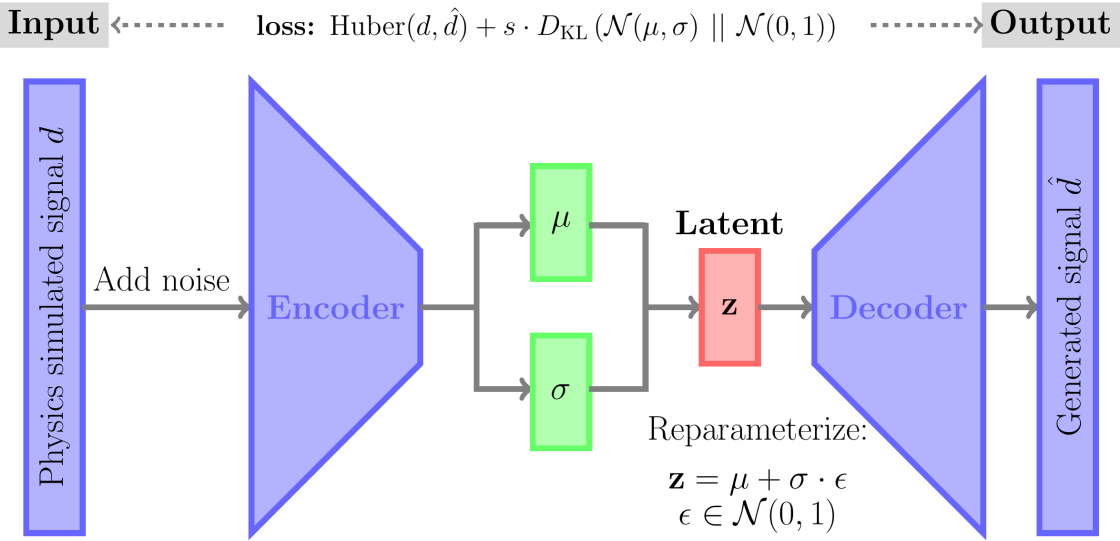
\includegraphics[width=\columnwidth]{../figures/fig1.png}
%		\caption{The architecture of a variational autoencoder.
%		}
%		\label{FIG:MODEL_VAE}
%	\end{figure}

	\subsection{Multi-Band Multi-Shot DWI Acquisition \& Modeling} \label{SEC:FWD}

	Our previous work \cite{tan_2024_naviepi} demonstrated
	the joint $k$-$q$-slice forward operator
	for multi-band multi-shot navigator-based interleaved EPI (NAViEPI) DWI acquisition.
	This operator can be understood as
	an extended sensitivity encoding (SENSE) operator \cite{pruessmann_2001_gsense},
	which maps the multi-slice multi-diffusion-weighted images ($\mathbf{x}$)
	to their corresponding $k$-space,
	\begin{equation}
		\mathcal{A}(\mathbf{x}) = \mathbf{P \Sigma \Theta F S \Phi} \mathbf{x}
		\label{EQU:FWD}
	\end{equation}
	Here, the images $\mathbf{x}$ are point-wise multiplied
	with the pre-computed shot-to-shot phase variation maps ($\mathbf{\Phi}$)
	and coil sensitivity maps ($\mathbf{S}$).
	The output images are then converted to $k$-space
	via two-dimensional fast Fourier transform ($\mathbf{F}$),
	point-wise multiplied with the multi-band phases ($\mathbf{\Theta}$),
	summed along the slice dimension ($\mathbf{\Sigma}$),
	and then multiplied by the $k$-space undersampling mask ($\mathbf{P}$).

	In \cref{EQU:FWD}, one challenge is
	to accurately estimate the shot-to-shot phase variation.
	Multiplexed sensitivity-encoding (MUSE) type reconstruction techniques
	\cite{liu_2004_diff_spiral,uecker_2009_nlinv_diff,chen_2013_muse,merrem_2019_nl_steam}
	achieved the self-gating strategy,
	where the $k$-space data of each shot were used to reconstruct
	its corresponding shot image followed by a phase smoothing approach.
	Self-gated shot phase estimation does not require
	the acquisition of phase navigator data.
	However, it requires small undersampling factors per shot and
	fully-sampled DWI acquisition assembling all shots.
	Alternatively, undersampled DWI acquisition can be enabled
	via the acquisition of navigators for shot phase estimation
	\cite{tan_2024_naviepi}.
	This approach allows for mesoscale-resolution DWI at \SI{7}{\tesla},
	but still needs long scan time.
	As listed in \cref{TAB:ACQ}, the total acquisition of
	Protocol \#1 at \SI{0.7}{mm} isotropic resolution
	takes $16:27$ minutes with phase navigators.
	This scan time can be reduced to approximately 10 minutes
	be removing the phase navigators (Protocol \#2 in \cref{TAB:ACQ}).
%	However, as mentioned above, self gating poses a constraint
%	on the achievable undersampling factor
%	for parallel imaging and compressed sensing reconstruction methods
%	(e.g., MUSE and joint reconstruction with LLR regularization).

	With the operator $\mathcal{A}$, the joint reconstruction is expressed as,
	\begin{equation}
		\argmin_{\mathbf{x}} \norm{\mathbf{y} - \mathcal{A}(\mathbf{x})}_2^2 + \lambda \mathcal{R}(\mathbf{x})
		\label{EQU:INV}
	\end{equation}
	where $\mathbf{y}$ is the measured $k$-space data.
	The first term in \cref{EQU:INV} presents the data-consistency term, and
	the second term presents the regularization function $\mathcal{R}(x)$
	with the regularization strength $\lambda$.
	When using the Tikhonov regularization,
	i.e.~$\mathcal{R}(\mathbf{x}) = \norm{\mathbf{x}}_2^2$,
	\cref{EQU:INV} can be solved via the conjugate gradient (CG) method.
	For nonlinear regularization functions,
	such as the locally-low rank (LLR) regularzation \cite{tan_2024_naviepi} or
	neural networks with nonlinear activation functions,
	ADMM was employed in this work to solve for \cref{EQU:INV}.

%	\subsection{Variational Autoencoder (VAE)}
%
%	Autoencoders comprise an encoder and a decoder, connected through a latent space.
%	Conventional autoencoders have no regularization
%	on the latent space.
%	Consequently, the learned latent space lacks meaningful
%	and structural representation.
%	To allow for dimension reduction while keeping the major part of
%	the data structure,
%	Kingma and Welling \cite{kingma_2014_vae} proposed
%	the variational autoencoder (VAE), as shown in \cref{FIG:MODEL_VAE}.
%	In VAE, the encoder maps each diffusion-weighted signal
%	into a Gaussian distribution ($\mathcal{N}(\mu, \sigma)$) within the latent space.
%	The latent variable ($\mathbf{z}$) is sampled according to the encoded distribution.
%	The decoder then maps the latent variable to the input space.
%	The training of a VAE uses the Huber loss together
%	with the Kullback-Leibler Divergence (KL-D).
%	The Huber loss minimizes the difference between the input and the output,
%	whereas KL-D minimizes the approximate posterior in latent space and
%	the exact posterior (assumed to be Gaussian distribution).


	\subsection{Algorithm Unrolling for Deep Image Reconstruction}

	Algorithm unrolling has been an emerging technique
	in solving inverse problems with learnable deep neural networks.
	Algorithm unrolling consists of two ingredients.
	First, it uses deep neural networks to learn regularization function.
	Second, it is constrained
	by the data-consistency term.
	In other words,
	the forward pass of the estimate $\mathcal{A} (\mathbf{x})$
	must be close to the measured data $\mathbf{y}$.
	By mapping the operations used in iterative algorithms
	onto neural networks, unrolled algorithms can be trained with data,
	leading to much faster inference
	than conventional iterative algorithms \cite{monga_2021_algunroll}.
	Further, recent developments have shown that
	the operations used in compressed sensing MRI,
	i.e., sparsifying transformation and soft thresholding,
	can be learned via neural networks.
	For instance, Hammernik et al.~\cite{hammernik_2018_varnet}
	proposed to unroll the gradient descent algorithm
	with a learned neural network
	(e.g.~U-Net \cite{ronneberger_2015_unet})
	as the regularization function.
	Aggarwal et al.~\cite{aggarwal_2018_modl} proposed
	the model-based deep learning architecture for inverse problems (MoDL)
	to unroll the alternating minimization algorithm
	with a learned residual denoising network (ResNet) \cite{he_2016_resnet}
	as regularization.


	\subsection{Self-Supervised Learning for High-Dimensional Image Reconstruction}

	In many HD-MRI applications, 
	such as dynamic imaging and diffusion-weighted imaging,
	acquiring fully-sampled data
	for supervised learning can be challenging.
	Recently, Yaman et al.~\cite{yaman_2020_ssdu}
	proposed self-supervised learning via data undersampling (SSDU) 
	for two-dimensional parallel imaging reconstruction.
	SSDU learns the regularization function in \cref{EQU:INV}
	by splitting available undersampled data into two disjoint sets,
	one of which is used in the data consistency term and
	another used for the computation in the training loss function.
	The training of SSDU requires large undersampled data sets.
	To close the domain gap between training and test data,
	Yaman et al.~\cite{yaman_2022_zs} proposed
	scan-specific zero-shot self-supervised learning (ZSSSL),
	which splits a single undersampled data set into three disjoint sets
	for (a) the data consistency term, (b) the loss calculation during training,
	and (c) validation, respectively.
	The concept of ZSSSL has been adopted for simultaneous 
	$T_1$ and $T_2$ relaxation parameter mapping
	\cite{heydari_2024_jmaple}.

	% ============================== %
	\section{Methods}

	\newcolumntype{a}{p{0.30\columnwidth}}
	\newcolumntype{b}{p{0.24\columnwidth}}
	\begin{table}
		\centering
		\caption{NAViEPI acquisition protocols}
		\label{TAB:ACQ}
		\begin{tabular}{a | b b}
			\toprule
			\textbf{Protocol} & \textbf{\#1} & \textbf{\#2} \\
			\hline
			Diffusion mode & \multicolumn{2}{c}{MDDW} \\
			Diffusion scheme & \multicolumn{2}{c}{monopolar} \\
			Diffusion direction & \multicolumn{2}{c}{$20$} \\
			$b$-value (\si{s/mm^2}) & \multicolumn{2}{c}{$1000$} \\
			$b_0$ & \multicolumn{2}{c}{$1$} \\
			FOV (\si{\square\mm}) & \multicolumn{2}{c}{$200$} \\
			Matrix size & \multicolumn{2}{c}{$286\times286\times176$} \\
			Voxel (\si{\cubic\mm}) & \multicolumn{2}{c}{$0.7\times0.7\times0.7$} \\
			Shots & \multicolumn{2}{c}{$3$} \\
			Acceleration & \multicolumn{2}{c}{$2 \times 2$} \\
			Partial Fourier & \multicolumn{2}{c}{$5/8$} \\
			Bandwidth (\si{Hz/Pixel}) & \multicolumn{2}{c}{$972$} \\
			ESP (\si{\ms}) & \multicolumn{2}{c}{$1.17$} \\
			Navigator & Yes & No \\
			TE (\si{\ms}) & $58/98.3$ & $58$ \\
			TR (\si{\ms}) & $15000$ & $8900$ \\
			Acquisition (\si{\minute}) & $16:27$ & $9:57$ \\
			\bottomrule
		\end{tabular}

%		\begin{tabular}{a | b b b}
%			\toprule
%			\textbf{Protocol} & \textbf{\#1} & \textbf{\#2} & \hl{\textbf{\#3}}\\
%			\hline
%			Diffusion mode & \multicolumn{3}{c}{MDDW} \\
%			Diffusion scheme & \multicolumn{3}{c}{monopolar} \\
%			Diffusion direction & \multicolumn{3}{c}{$20$} \\
%			$b$-value (\si{s/mm^2}) & \multicolumn{3}{c}{$1000$} \\
%			$b_0$ & \multicolumn{3}{c}{$1$} \\
%			FOV (\si{\square\mm}) & \multicolumn{3}{c}{$200$} \\
%			Matrix size & \multicolumn{3}{c}{$286\times286\times176$} \\
%			Voxel (\si{\cubic\mm}) & \multicolumn{3}{c}{$0.7\times0.7\times0.7$} \\
%			Shots & \multicolumn{2}{c}{$3$} & $6$ \\
%			Acceleration & \multicolumn{2}{c}{$2 \times 2$} & $1 \times 2$ \\
%			Partial Fourier & \multicolumn{3}{c}{$5/8$} \\
%			Bandwidth (\si{Hz/Pixel}) & \multicolumn{2}{c}{$972$} & $1166$\\
%			ESP (\si{\ms}) & \multicolumn{2}{c}{$1.17$} & $1.11$ \\
%			Navigator & Yes & No & No \\
%			TE (\si{\ms}) & $58/98.3$ & $58$ & $56$ \\
%			TR (\si{\ms}) & $15000$ & $8900$ & $9000$ \\
%			Acquisition (\si{\minute}) & $16:27$ & $9:57$ & $19:27$ \\
%			\bottomrule
%		\end{tabular}
	\end{table}

	\subsection{Data Acquisition}

	\cref{TAB:ACQ} lists two acquisition protocols implemented on
	a clinical \SI{7}{\tesla} MR system
	(MAGNETOM Terra, Siemens Healthineers, Erlangen, Germany)
	equipped with a 32-channel head coil (Nova Medical, Wilmington, MA, USA)
	and the XR-gradient system
	(maximum gradient strength \SI{80}{\milli\tesla/\meter} and
	a peak slew rate \SI{200}{\tesla/\meter/\second}).
	Protocols \#1 and \#2 realized mesoscale high-resolution DWI with \SI{0.7}{mm}
	isotropic resolution. Two-fold acceleration is employed
	in both in-plane and slice directions.
	Every DWI data is acquired by three shots in an interleaved manner,
	which resultes in $6 \times 2$-fold acceleration per shot.
	Noteworthy, the total scan time can be reduced to about 10~minutes
	(Protocol \#2) when switching off navigator acquisition.
	Three young healthy volunteers with written informed consent
	approved by the local ethics committee
	participated in this study.

	\subsection{Image Reconstruction via ADMM Unrolling}

	\begin{algorithm}
		\caption{Self-Supervised ADMM Unrolling} \label{ALG:ADMM}
		\begin{algorithmic}[1]
			\State \textbf{Initialization}:
			\State \;\; split sampling mask $\mathbf{P}$ into 12 repetitions, each of which consists of three disjoint sets $\mathbf{T}$, $\mathbf{L}$, and $\mathbf{V}$
			\State \;\: $p \gets 0$ and $N_{\mathrm{epoch}} \gets 100$
			\State \;\; $\mathcal{D}_{\omega}$ set as ResNet
			\State \;\; $\rho \gets 0.05$ and $\lambda \gets 0.05$
			\State \;\; $\mathrm{Loss}_{\mathrm{valid}} \gets \inf$ and $\mathrm{trace} \gets 0$
			\Function{ADMM}{$\mathrm{mask}$}
			\State $\mathcal{A}_\mathrm{mask} \gets$ set the mask in the forward operator $\mathcal{A}$
			\State $\mathbf{x}^{(0)} \gets \mathcal{A}_\mathrm{mask}^H (\mathbf{y})$
			\State $\mathbf{v}^{(0)} \gets \mathbf{x}^{(0)}$ and $\mathbf{u}^{(0)} \gets \mathbf{0}$
			\State $k \gets 0$ and $N_{\mathrm{unroll}} \gets 8$
			\While{$k < N_{\mathrm{unroll}}$}
			\State $\mathbf{x}^{(k+1)} \gets $ conjugate gradient with 6 iterations
			\State $\mathbf{v}^{(k+1)} \gets (\lambda/\rho) \cdot \mathcal{D}_{\omega} (\mathbf{x}^{(k+1)} + \mathbf{u}^{(k)})$
			\State $\mathbf{u}^{(k+1)} \gets \mathbf{u}^{(k)} + \mathbf{x}^{(k+1)} - \mathbf{v}^{(k+1)}$
			\State $k \gets k+1$
			\EndWhile
			\State \Return $\mathbf{x}^{(k+1)}$
			\EndFunction
			\State \textbf{Training}:
			\While{$p < N_{\mathrm{epoch}}$ or $\mathrm{trace} \leq 12$}
			\State $\mathbf{x}_t \gets \mathrm{ADMM}(\mathbf{T})$
			\State $\mathrm{Loss}_{\mathrm{train}} \gets \mathcal{L}(\mathbf{L} \mathbf{y}, \mathcal{A}_\mathbf{L}(\mathbf{x}_t))$
			\State update $\omega$ via ADAM
			\State \textbf{Validation}:
			\State $\mathbf{x}_t \gets \mathrm{ADMM}(\mathbf{T} \cup \mathbf{L})$
			\State $\mathrm{Loss}_{\mathrm{temp}} \gets \mathcal{L}(\mathbf{V} \mathbf{y}, \mathcal{A}_\mathbf{V}(\mathbf{x}_t))$
			\If{$\mathrm{Loss}_{\mathrm{temp}} \leq \mathrm{Loss}_{\mathrm{valid}}$}
			\State $\mathrm{Loss}_{\mathrm{valid}} \gets \mathrm{Loss}_{\mathrm{temp}}$
			\State $\mathrm{trace} \gets 0$
			\Else
			\State $\mathrm{trace} \gets \mathrm{trace} + 1$
			\EndIf
			\EndWhile
		\end{algorithmic}
	\end{algorithm}

	\begin{figure}
		\centering
		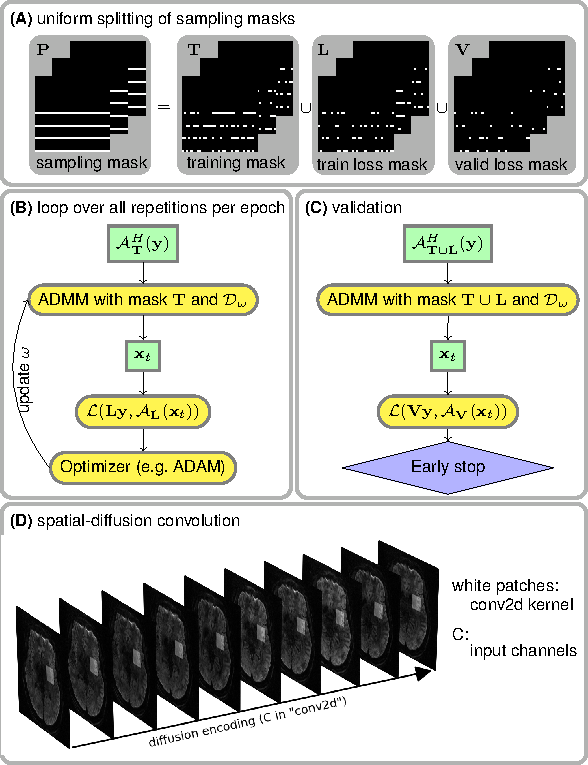
\includegraphics[width=\columnwidth]{../figures/fig1.pdf}
		\caption{Illustration of the key components in ADMM unrolling.
			\textbf{(A)} The sampling mask $P$ in \cref{EQU:FWD} was
			uniformly split into three disjoint sets:
			the training mask $\mathbf{T}$ used for
			the data consistency term during training,
			the train loss mask $\mathbf{L}$ used for
			the loss function calculation during training, and
			the validation loss mask $\mathbf{V}$ used for
			the loss function calculation during validation.
			\textbf{(B)} and \textbf{(C)} show the flowchart
			for the training and the validation of an unrolled ADMM model, respectively.
			Note that the ResNet parameters $\omega$ are updated 
			via ADAM \cite{kingma_2015_adam} during training,
			but remain fixed during the validation step.
			\textbf{(D)} A stack of diffusion-weighted images 
			is input into ResNet during ADMM unrolling.}
		\label{FIG:ZSSSL}
	\end{figure}

	Instead of the two-step alternating minimization unrolling scheme as used in MoDL
	\cite{aggarwal_2018_modl},
	we employed the ADMM unrolling
	to solve the self-supervised learning reconstruction
	in \cref{EQU:INV}. The update rule of ADMM unrolling reads
	\begin{equation} \label{EQU:ADMM}
		\left\{\begin{aligned}
			\mathbf{x}^{(k+1)} &= \argmin_{\mathbf{x}^{(k)}} \norm{\mathbf{y} - \mathcal{A}(\mathbf{x}^{(k)})}_2^2 + \frac{\rho}{2} \norm{ \mathbf{x}^{(k)} - \mathbf{v}^{(k)} + \mathbf{u}^{(k)}}_2^2 \\
			\mathbf{v}^{(k+1)} &= (\lambda/\rho) \cdot \mathcal{D}_{\omega} (\mathbf{x}^{(k+1)} + \mathbf{u}^{(k)}) \\
			\mathbf{u}^{(k+1)} &= \mathbf{u}^{(k)} + \mathbf{x}^{(k+1)} - \mathbf{v}^{(k+1)}
		\end{aligned}\right.
	\end{equation}
	ADMM updates the variables $\mathbf{x}$, $\mathbf{v}$,
	and $\mathbf{u}$ in an alternating scheme.
	It splits the unrolled reconstruction into three steps,
	as shown in \cref{EQU:ADMM} and in the pseudo code of \cref{ALG:ADMM}.
	First, the updating step for $\mathbf{x}$ is solved by conjugate gradient.
	Second, the variable $\mathbf{v}$ is then updated
	via the forward pass of the neural network $\mathcal{D}_{\omega}$
	with the input as the sum of current estimates
	of $\mathbf{x}$ and $\mathbf{u}$.
	Third, the variable $\mathbf{u}$ is updated
	by adding its current estimate to the difference
	between $\mathbf{x}$ and $\mathbf{v}$.

	As shown in \cref{FIG:ZSSSL}, to train an unrolled ADMM model, 
	the data sampling mask $\mathbf{P}$
	is split into three disjoint sets, 
	the training mask $\mathbf{T}$ for the data consistency term,
	the training loss mask $\mathbf{L}$ for the loss function calculation,
	and the validation loss mask $\mathbf{V}$.
	Each set consists of 12 repetitions constructed via random uniform sampling
	of the data mask $\mathbf{P}$.
	In each training epoch, every repetition is looped through
	in order to update the ResNet parameters $\omega$.
	Plus, the validation step is performed after every training epoch
	to update the minimal validation loss.
	If the validation loss does not reduce for 12 consecutive epochs or
	if 100 epochs are reached, the training is terminated.

	The index $k$ in \cref{EQU:ADMM} denotes the unrolling iteration,
	and $\mathcal{D}_{\omega}$ denotes the ResNet \cite{he_2016_resnet}
	parameterized by $\omega$.
	In this work, 2D convolution was employed to construct the ResNet layers.
	In PyTorch, 2D convolution requires four-dimensional tensors as input and output.
	For instance, a matrix with the size $(N, C, H, W)$ is acceptable
	for the the 'conv2d' function in PyTorch.
	Here, $W$ and $H$ denote the width and height of the convolution kernel,
	$C$ denotes the number of channels, and $N$ denotes the batch size.
	However, the diffusion-weighted images ($\mathbf{x}$) to be reconstructed
	has the size $(N_{\text{diff}}, N_Z, N_Y, N_X, 2)$,
	where $2$ stands for the real and imaginary part 
	of the complex-valued diffusion-weighted images,
	$N_X$ and $N_Y$ are the width and the height of diffusion-weighted images,
	$N_Z$ is the number of slices (identical to the multi-band factor), and
	$N_{\text{diff}}$ is the number of diffusion encoding.
	To train a ResNet based on 2D convolution, 
	the diffusion-weighted images were reshaped and permuted
	as $(N_Z, 2 \cdot N_{\text{diff}}, N_Y, N_X)$, as illustrated in \cref{FIG:ZSSSL} (D).
	In this manner, 2D convolution kernels in combination with ReLU activation functions
	loop through the varying diffusion-weighted contrast
	to learn the key features of the high-dimensional data and
	to reduce noisy and aliasing artifacts in unrolled reconstruction.
	
	\subsection{Model Generalizability} \label{SEC:ZSSSL_GEN}
	
	Volumetric whole brain DWI acquisition consists of many multi-band slices, 
	and the training of algorithm unrolling models on all slices requires 
	hundreds of GPU computing hours. 
	To investigate the model generalizability and to accelerate reconstruction, 
	we performed two training and inference strategies. 
	First, we trained the ADMM unrolling model with only one multi-band slice data, 
	and then tested the model on all remaining multi-band slices. 
	We dubbed this approach as "single-slice training". 
	Second, we trained and tested every multi-band slice individually, 
	which was dubbed as "slice-by-slice training". 
	The single-slice training strategy saves tremendous computing time, 
	as its model is learned from one single slice and 
	the inference time per slice is only about one minute. 
	By comparing these two training strategies, 
	we aim at demonstrating the model generalizability and 
	its applicability to other slices which are "unseen" in single-slice training.

	\subsection{Self-Gated ADMM Unrolling}

	As discussed in \cref{SEC:FWD}, there are two approaches for
	estimating shot-to-shot phase variation: self-gated and navigator-based.
	The self-gated approach, as used in MUSE \cite{chen_2013_muse},
	requires fully-sampled DWI acquisition and
	has typically reported only a small number of shots (up to 4).
	The previously proposed NAViEPI approach enabled high-resolution DWI
	with the use of undersampled iEPI and shot-to-shot phase navigator acquisition.
	While NAViEPI results in shorter scan time than fully-sampled iEPI,
	the use of phase navigator still elongates the acquisition,
	as listed in \cref{TAB:ACQ}.
	Therefore, a key question is whether it is feasible to
	discard the shot-to-shot phase navigator 
	while keeping undersampled iEPI acquisition.
	In this work, we investigated the feasibility of ADMM unrolling in self-gated scan
	for \SI{0.7}{\milli\meter} isotropic resolution DWI.

	\subsection{Comparison of Regularization Techniques}
	
	This work compared the reconstruction performance
	of three different regularization techniques,
	Tikhonov $\ell^2$ regularization (as used in MUSE),
	LLR regularization,
	and ADMM unrolling with a learned regularization.
	Note that MUSE is a simultaneous multi-slice (SMS) parallel imaging method
	and poses no regularization along the diffusion dimension,
	effectively solving each DWI reconstruction independently.
	In contrast, all the other two regularized reconstructions
	fall into the joint reconstruction regime.
	They jointly reconstruct all diffusion-weighted images
	and impose regularization terms exploring spatial-diffusion redundancies.
	For example, LLR enforces the low rankness of
	local spatial-diffusion matrices from diffusion-weighted images,
	whereas ADMM unrolling learns a regularization function composed by neural networks
	based on spatial-diffusion convolution kernels
	while enforcing data consistency during the unrolled training process.

	\subsection{Computation}

	All reconstructions in this work were done on a single A100 SXM4/NVLink GPU
	with \SI{80}{\giga\byte} memory (NVIDIA, Santa Clara, CA, USA).
	Computing infrastructure was provided by
	the Erlangen National High Performance Computing Center and 
	by the Advanced Research Computing at the University of Michigan, Ann Arbor.

	% ============================== %
	\section{Results}

	\subsection{Model Generalizability}
	
	\begin{figure*}
		\begin{minipage}[c]{0.75\textwidth}
			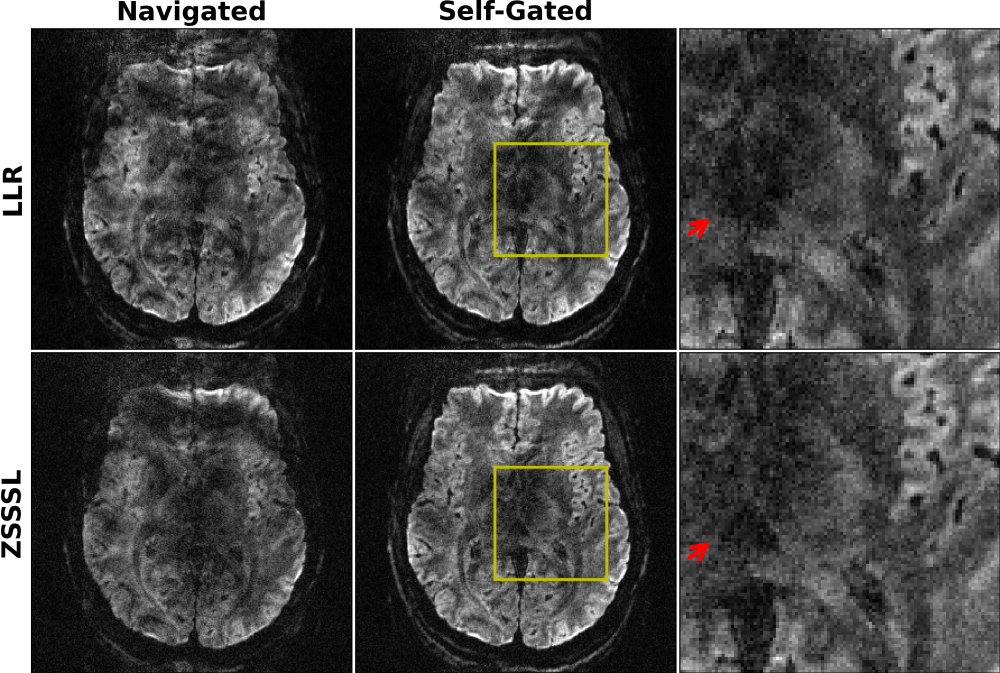
\includegraphics[width=\textwidth]{../figures/fig2.png}
		\end{minipage}\hfill
		\begin{minipage}[c]{0.23\textwidth}
			\caption{Comparison of two training strategies: 
				(1) slice-by-slice training, 
				where every slice is trained and tested individually; 
				(2) single-slice training, 
				where the unrolled ADMM model is trained on only one slice 
				and tested on all remaining slices.
				The top-right image shows the absolute difference 
				between the reconstructed diffusion-weighted images 
				at the 10th diffusion direction 
				between (1) and (2). 
				The bottom panel plots the mean and standard deviation 
				of the signal within yellow and green rectangles 
				in the slide-by-slice training and the single-slice training, 
				respectively. 
				No major qualitative or quantitative difference can be seen 
				between the two training strategies.}
			\label{FIG:GENERALIZATION}
		\end{minipage}
	\end{figure*}
	
	\cref{FIG:GENERALIZATION} demonstrates the generalizability 
	of the proposed ADMM unrolling approach, 
	i.e., an unrolled ADMM model trained on one single slice 
	is applicable to all remaining "unseen" slices. 
	Single-direction diffusion-weighted images from 
	both the slice-by-slice training 
	and the single-slice training strategies are displayed. 
	The absolute difference between these two images 
	shows no residual structural information, but mainly noise.
	Further, we plotted the mean and standard deviation 
	within the selected region-of-interest (colored boxes in \cref{FIG:GENERALIZATION}) 
	along all diffusion encoding.
	This again proves the cross-slice generalization 
	of the proposed ADMM unrolling method.
	The plotted curves show quantitatively similar values 
	between the two training strategies.
	With this, all following results were obtained 
	utilizing the single-slice training strategy.

	\subsection{Retrospectively Self-Gated ADMM Unrolling}

	\begin{figure*}
		\begin{minipage}[c]{0.75\textwidth}
			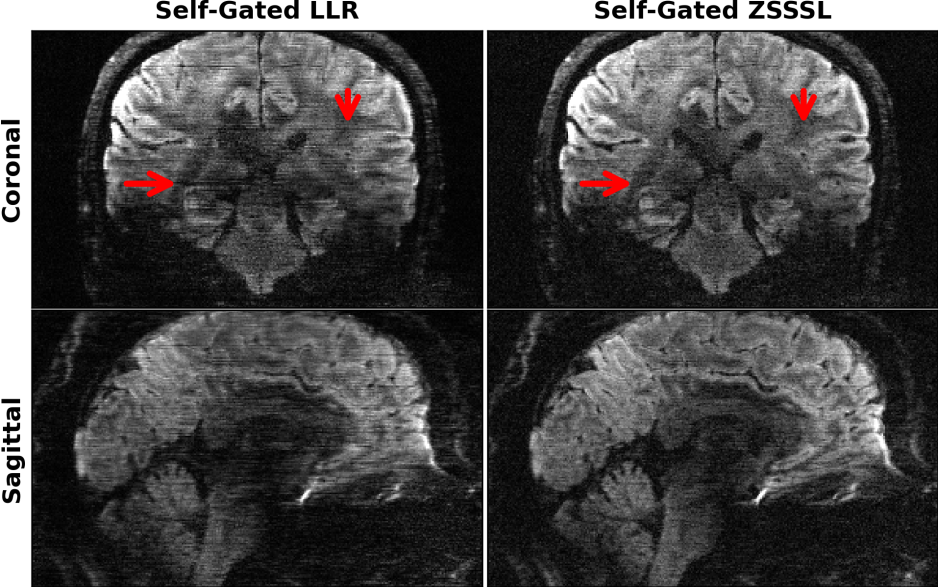
\includegraphics[width=\textwidth]{../figures/fig3.png}
		\end{minipage}\hfill
		\begin{minipage}[c]{0.23\textwidth}
			\caption{Comparison of (top) LLR regularized 
				and (bottom) ADMM unrolling
				reconstruction on 0.7~mm isotropic resolution DWI
				acquired by Protocol \#1
				with shot phase estimated from
				(left) navigators and (middle) imaging echoes, respectively.
				Zoomed views of the yellow boxes from the self-gated reconstruction
				are displayed in the right-most column.
				The use of navigators prolongs the total scan time,
				and thus increases the sensitivity to motion,
				as shown in the single-direction diffusion-weighted image 
				reconstructed with navigated shot phase, 
				where accidental motion occurred during navigator acquisition.
				The retrospectively self-gated reconstruction discards navigators,
				and renders sharper diffusion-weighted images. 
				Compared to LLR, unrolled ADMM is advantageous
				in resolving clearer tissue boundaries 
				in diffusion-weighted images,
				as indicated by red arrows.}
				\label{FIG:MOTION_RETRO_TRA}
		\end{minipage}
	\end{figure*}

	\cref{FIG:MOTION_RETRO_TRA} demonstrates
	the efficacy of the self-gated self-supervised ADMM unrolling reconstruction
	by comparing to the navigated and self-gated reconstructions 
	on the first volunteer.
	Data were acquired by the NAViEPI sequence, 
	as listed in Protocol \#1 in \cref{TAB:ACQ}.
	The single-direction diffusion-weighted images with accidental motion
	are displayed.

	The selected diffusion encoding shows residual aliasing-like and
	severe motion-blurring artifacts
	in the navigated reconstructions, 
	including both LLR regularization and ADMM unrolling.
	The main reason of these artifacts is that
	the acquisition of navigators
	increases the total scan time,
	resulting in higher sensitivity to accidental inter-shot motion.
	Admittedly, navigators are valuable 
	in the case of ultra high spatial resolution
	using many shots, e.g.~3-fold in-plane undersampling and 5-shot acquisition
	for the in-plane resolution of 0.5~mm \cite{tan_2024_naviepi}, 
	which led to an in-plane acceleration of $15$ per shot.
	In contrast, this experiment utilized 3 shots, yielding
	$6 \times 2$-fold acceleration per shot (refer to Protocol \#1).
	Such an acceleration rate proves achievable in the self-gated approach.
	Both LLR regularized and unrolled ADMM reconstructions supply geometrically correct 
	diffusion-weighted images
	without noticeable aliasing artifacts. 
	This in turn indicates that motion corrupted the navigator data 
	in this measurement.
	Further, self-gated ADMM unrolling exhibits much clearer tissue delineation
	in reconstructed diffusion-weighted images, 
	as indicated by red arrows in the zoomed-in views
	in \cref{FIG:MOTION_RETRO_TRA},
	whereas self-gated LLR suffers from
	slightly blurry tissue boundaries and ambiguous signals.

	\begin{figure*}
		\begin{minipage}[c]{0.75\textwidth}
			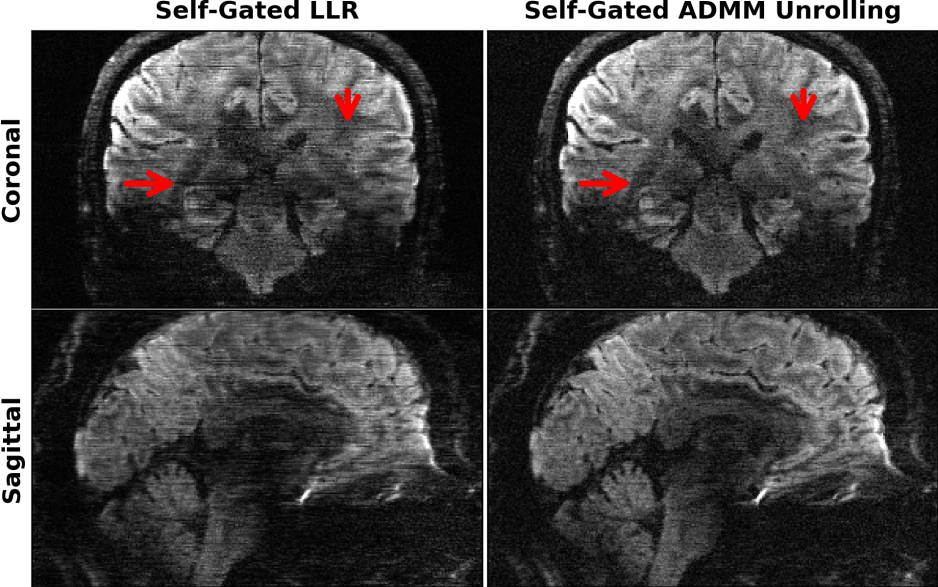
\includegraphics[width=\textwidth]{../figures/fig4.png}
		\end{minipage}\hfill
		\begin{minipage}[c]{0.23\textwidth}
			\caption{Single-direction diffusion-weighted images 
				at 0.7~mm isotropic resolution
				as reconstructed by retrospectively self-gated
				(left) LLR and (right) ADMM unrolling
				in (top) the coronal and (bottom) the sagittal views, respectively.
				The same diffusion direction as in \cref{FIG:MOTION_RETRO_TRA}
				is chosen for display.
				ADMM unrolling reduces phase ambiguities 
				in the shot-combined reconstruction, 
				thereby rendering clearer tissue delineation and
				reducing stripping artifacts (as indicated by the red arrows).}
			\label{FIG:MOTION_RETRO_2}
		\end{minipage}
	\end{figure*}

	\cref{FIG:MOTION_RETRO_2} shows coronal- and saggital-view 
	diffusion-weighted images
	with the same diffusion encoding as in \cref{FIG:MOTION_RETRO_TRA}.
	As mentioned in \cref{SEC:ZSSSL_GEN}, the unrolled ADMM model 
	was trained using only one slice
	and then inferred on all remaining slices.
	The model generalizes well across slices.
	The inference of every slice takes only about one minute,
	whereas the LLR reconstruction takes about 48~minutes per slice.
	More importantly, the self-gated LLR reconstruction exhibits residual
	motion-induced stripping artifacts 
	(refer to red arrows in \cref{FIG:MOTION_RETRO_2}) \cite{chang_2021_musium},
	whereas the self-gated ADMM unrolling approach substantially removes these artifacts
	and supplies high-quality diffusion-weighted images without the need of navigators.
	Both reconstructions show $B_1$ field inhomogeneities in the cerebellum region 
	and residual spatial distortion in the frontal brain region. 
	These artifacts, however, are beyond the scope of this work.
	

	\subsection{Prospectively Self-Gated ADMM Unrolling}

	\begin{figure*}
		\centering
		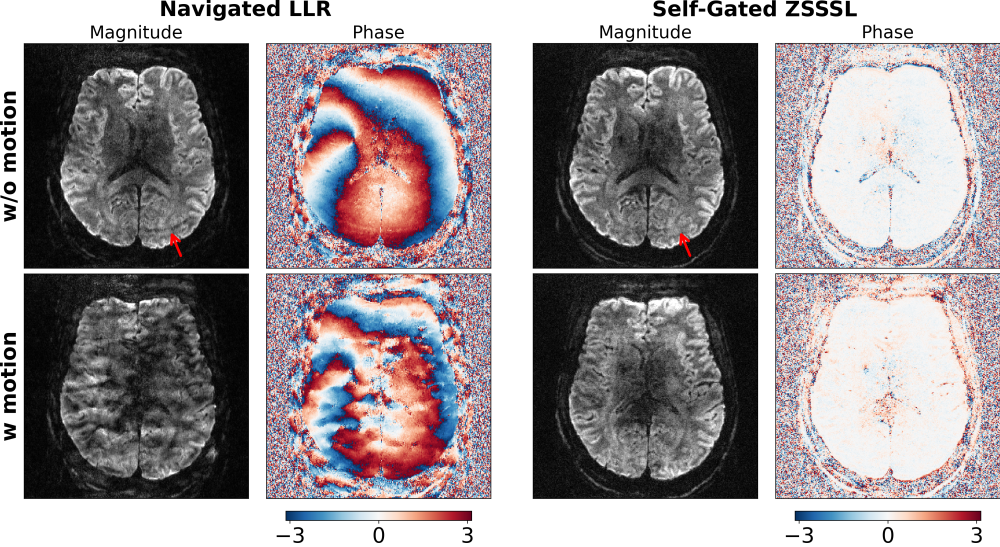
\includegraphics[width=\textwidth]{../figures/fig5.png}
		\caption{0.7~mm isotropic mesoscale DWI with 21 volumes at about 10~minutes
			without the acquisition of navigators.
			(A) Single-direction diffusion-weighted images and
			(B) Mean diffusion-weighted images of 20 diffusion directions
			at three orthogonal orientations are displayed.
			Diffusion-weighted images were reconstructed by
			(top) MUSE, (middle) LLR, and (bottom) ADMM unrolling.
			MUSE suffers from severe noise artifacts at such small voxel size.
			LLR is able to clean up most of the noise,
			but is still hampered by signal void artifacts in the axial view,
			which appears as stripping artifacts in coronal and sagittal views
			(as indicated by red arrows).
			ADMM unrolling significantly reduces both noise and signal voids.
			In the mean diffusion-weighted images, LLR shows amplified noise
			in the cerebellum region (see the blue arrow in the sagittal view),
			whereas ADMM unrolling yields more homogeneous signal distributions.}
		\label{FIG:MOTION_PROS}
	\end{figure*}

	\cref{FIG:MOTION_PROS} compares the reconstruction results
	using the prospectively acquired iEPI data without navigators
	of the second volunteer
	(refer to Protocol \#2 in \cref{TAB:ACQ}).
	The snapshot single diffusion-direction diffusion-weighted images
	as well as mean diffusion-weighted images 
	at three orthogonal views were displayed.
	
	The MUSE reconstruction suffers from strong noise
	at such mesoscale voxel size. 
	Its corresponding mean diffusion-weighted images show 
	improved the visibility of brain tissues, 
	but the overall image quality is not sufficient.
	The LLR regularized reconstruction largely reduces noise,
	but still exhibits suspicious dark signal in the axial view,
	which appears as striping artifacts in the coronal and the sagittal views
	(refer to the red arrows in \cref{FIG:MOTION_PROS}).
	On the other hand, the LLR regularized reconstruction
	shows amplified noise in the cerebellum region
	(refer to the blue arrow in the sagittal view of \cref{FIG:MOTION_PROS}),
	which could be caused by the $B_1$ excitation field inhomogeneity
	at \SI{7}{\tesla}.	

	The above-mentioned striping artifacts are nearly gone 
	in the unrolled ADMM reconstruction.
	Moreover, the diffusion-weighted images from ADMM unrolling in the axial view 
	show clearer diffusion contrasts 
	and thus better tissue delineation and continuity 
	in the coronal and the sagittal views.
	Further, as indicated by the blue arrows in \cref{FIG:MOTION_PROS},
	the diffusion-weighted image in the sagittal view shows more homogeneous
	signal distribution and reduced noise surrounding the cerebellum.

	\begin{figure}
		\centering
		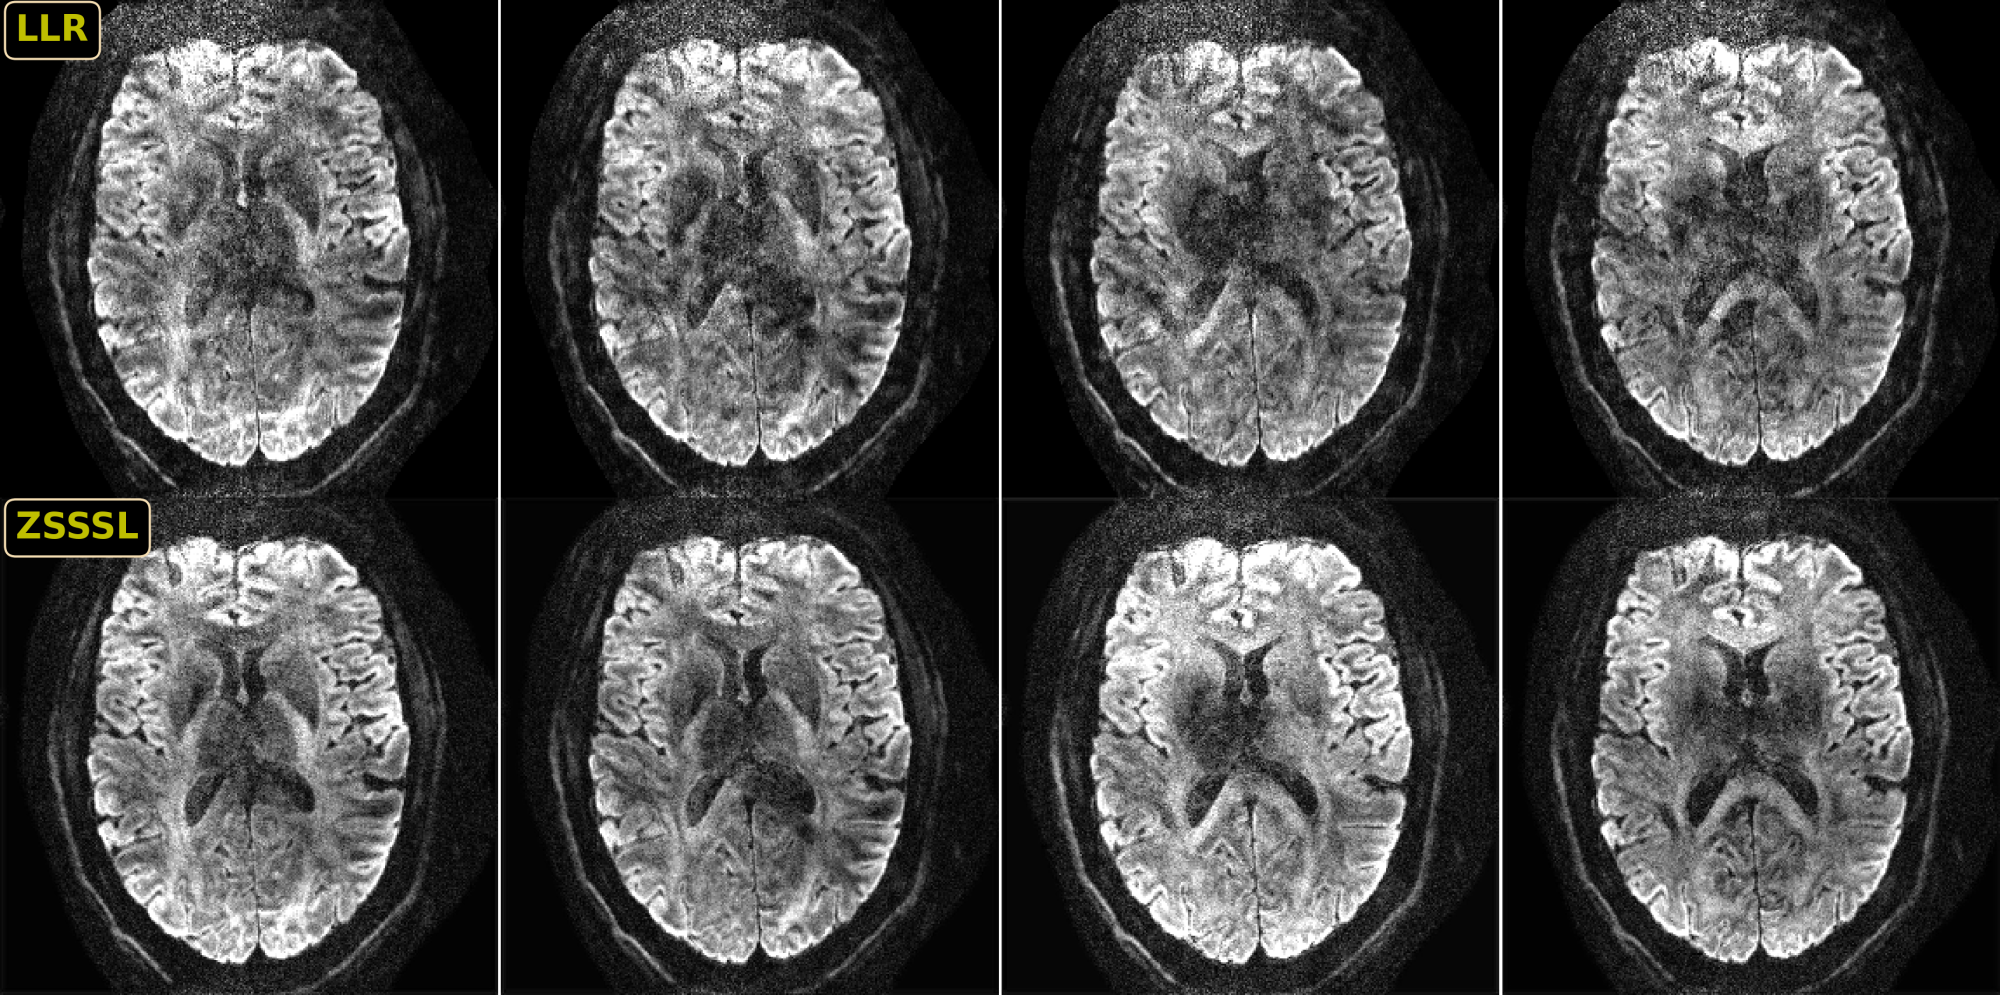
\includegraphics[width=\columnwidth]{../figures/fig6.png}
		\caption{Convergence analysis along the ADMM unrolling training
			and validation epochs
			for the results in \cref{FIG:MOTION_PROS}.
			Displayed curves are (red solid) the training loss,
			(red dashed) the validation loss,
			and (blue solid) the learned regularization strength $\lambda$, respectively.
			All parameters converge sufficiently and show no over-fitting.}
		\label{FIG:CONVERGENCE}
	\end{figure}

	\cref{FIG:CONVERGENCE} displays the training and validation loss
	as well as the learned regularization strength along epochs 
	for the results shown in \cref{FIG:MOTION_PROS}.
	It can be seen that 100 epochs are sufficient for
	the convergence of ADMM unrolling. 
	The model converges well along epochs, 
	and does not show any over-fitting behavior 
	(The validation loss decays similarly as the training loss).
	In addition, the regularization strength converges
	to the value of about 0.027.

	\begin{figure*}
		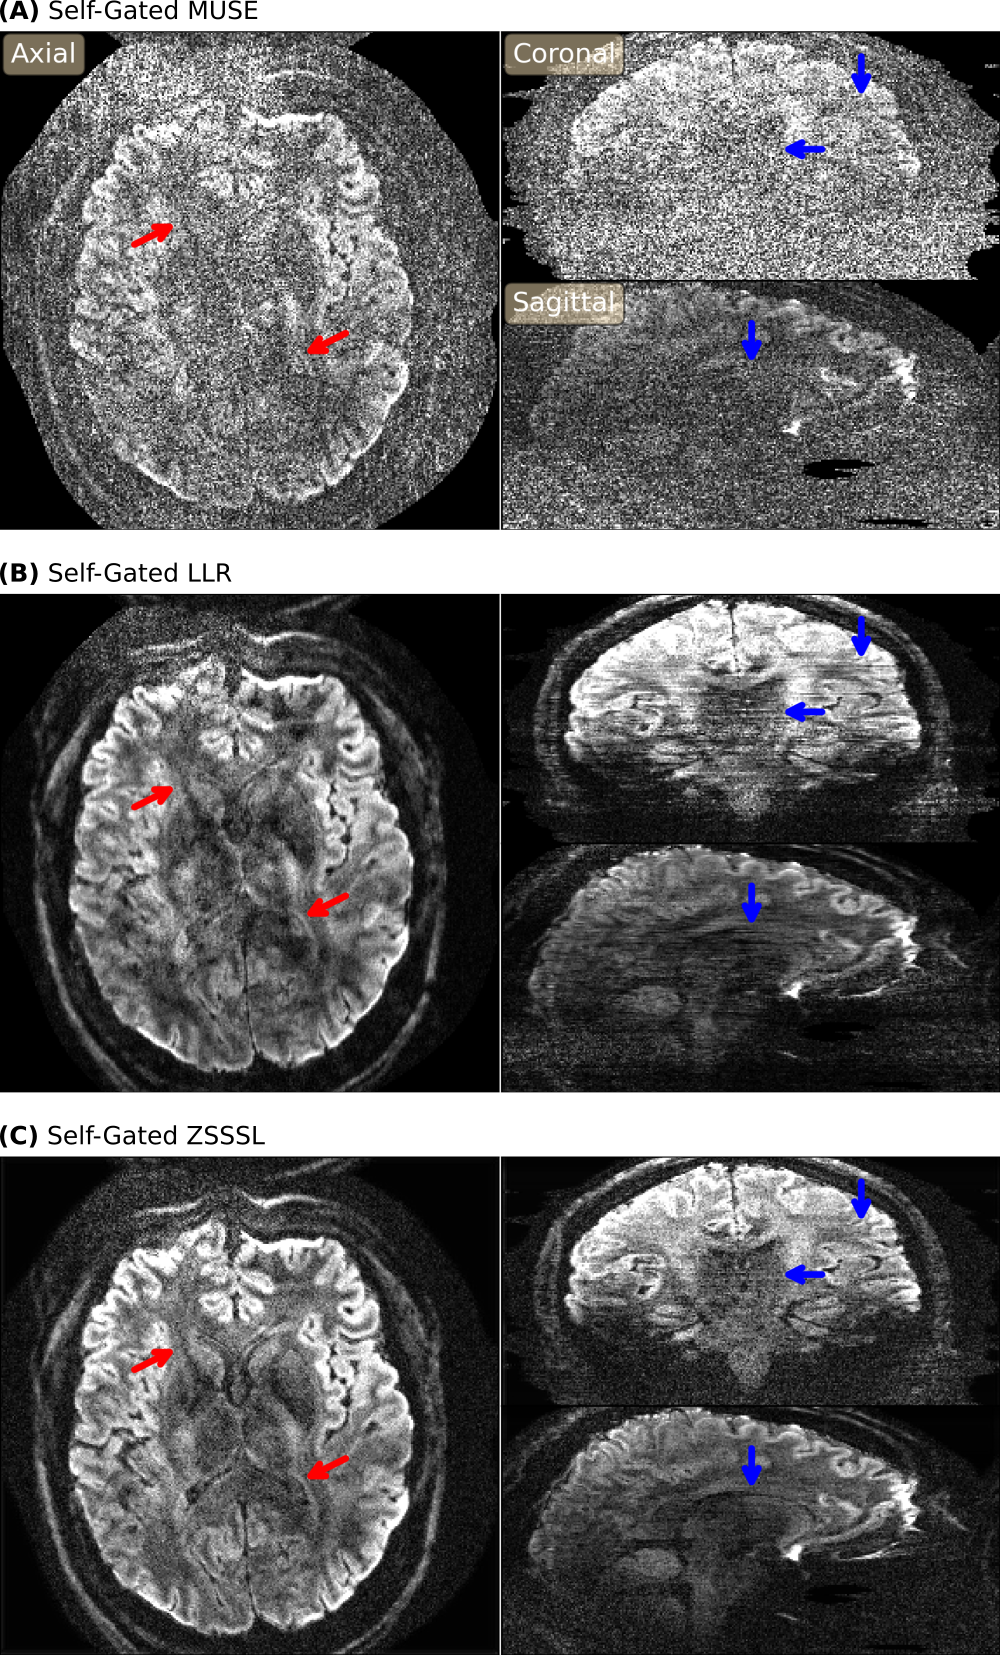
\includegraphics[width=\textwidth]{../figures/fig7.png}
		\caption{Prospectively self-gated DWI reconstruction results
			at 0.7~mm isotropic resolution. Displayed images are
			one axial slice at four different diffusion-encoding directions.
			ADMM unrolling enables much cleaner delineations of diffusion contrasts
			than LLR regularized reconstruction.}
		\label{FIG:SG_ZSSSL_VOL3}
	\end{figure*}

	\cref{FIG:SG_ZSSSL_VOL3} shows the reconstructed diffusion-weighted images
	at four different diffusion directions based on the iEPI data
	acquired from the third volunteer 
	(the same subject as in \cref{FIG:GENERALIZATION}).
	In this experiment, the volunteer was instructed
	to keep still during scan.
	Again, the proposed self-gated ADMM unrolling reconstruction
	with spatial-diffusion convolution illustrates
	superior tissue structure delineation and 
	diffusion contrasts
	to the LLR regularized reconstruction. 
	The LLR reconstruction suffers from 
	amplified noise in the frontal brain region.
	In contrast, the unrolled ADMM approach generally illustrates 
	more homogeneous signal and noise distribution 
	across the field-of-view. 
	While LLR builds upon one single linear transformation 
	(singular-value decomposition, SVD) and 
	one nonlinear operation (soft thresholding) \cite{cai_2010_svt}, 
	the ResNet in ADMM unrolling builds upon 
	multiple two-dimensional convolutions and nonlinear activation functions. 
	Therefore, deep neural networks enable more in-depth exploration 
	of key features in the high-dimensional data.



	% ============================== %
	\section{Discussion}

	This work reported a novel self-gated self-supervised learning approach 
	based on ADMM unrolling
	for multi-shot undersampled iEPI acquisition and high-resolution DWI reconstruction.
	The self-gated ADMM unrolling achieved whole brain DWI 
	with 20 diffusion-encoded directions and a $b$-value of \SI{1000}{s/mm^2}
	at \SI{0.7}{mm} isotropic resolution,
	all within a scan time of less than 10 minutes.
	For comparison, the compressed sensing reconstruction with 
	locally-low rank regularization was implemented also with the generic ADMM algorithm.
	Thus, our work assured fair comparison among different regularization methods.

	The proposed self-gated ADMM unrolling approach is well-suited 
	for online reconstruction deployment.
	Firstly, it requires much shorter acquisition time than
	the conventional MUSE approach with fully-sampled iEPI and
	our previous NAViEPI method.
	Secondly, it does not require large-scale fully-sampled data for training.
	Instead, its training is scan specific and requires only one slice.
	The trained ADMM unrolling model is applicable to different slices.
	Third, the inference time of the trained model is much
	shorter compared to the LLR regularization approach.

	We observed that stripping-type motion artifacts occurred more frequently
	in the sub-millimeter isotropic resolution DWI regime.
	In addition, sub-millimeter isotropic voxel 
	resulted in higher noise in diffusion-weighted images.
	This makes sense, as scans with reduced slice thickness are more susceptible to
	shot-to-shot phase variations.
	To enable sub-millimeter mesoscale DWI,
	Setsompop et al.~\cite{setsompop_2018_gslider}
	proposed the gSlider technique with slice phase–dither encoding,
	which excites one slab multiple times with complementary slice encoding schemes.
	gSlider has been proven effective in alleviating motion sensitivity,
	because the thicker slab (in comparison to the thin single slice)
	reduced inter-slice motion.
	Meanwhile, Hadamard encoding of the slices within a slab gained SNR
	in the linear inverse reconstruction.
	However, it has been reported that gSlider has stricter requirements
	on $B_0$ and $B_1$ field homogeneities 
	and shows residual slab boundary artifacts
	\cite{dai_2021_smslab}.
	In contrast, the proposed self-gated self-supervised ADMM unrolling method
	requires no such advanced slab encoding,
	while achieves sub-millimeter resolution
	at a clinical feasible reconstruction time.
	Thus, the proposed method can be useful for the probe to high-resolution
	brain micro-structures in the human connectome project \cite{huang_2021_hcp2}.
	On the other hand, since unrolled algorithms are flexible to 
	MR physics modeling (e.g., the forward operator $\mathcal{A}$), 
	the proposed ADMM unrolling can be extended 
	to incorporate with the gSlider encoding model for enhanced SNR performance.

	This work demonstrated the capability of self-gated ADMM unrolling in
	reconstructing \SI{0.7}{mm} isotropic resolution 3-shot iEPI DWI
	with $(6 \times 2)$-fold acceleration per shot.
	However, we also observed that the self-gated approach
	failed to recover aliasing-free diffusion-weighted images
	in the case of higher acceleration factors
	(e.g. the $0.5\times0.5\times2.0$~\si{mm^3} DWI data
	with an acceleration of $15\times2$ per shot).
	To address this issue, acquiring shot-to-shot phase navigators 
	helps with the shot-combined DWI reconstruction \cite{tan_2024_naviepi}.
	Therefore, the utilization of navigator acquisition and 
	advanced deep learning reconstruction should be application oriented.
	For ultra-high spatial resolution that requires many shots, 
	navigator is needed. 
	For the 0.7~mm resolution with 3 shots as shown in this work,
	the self-gated acquisition is beneficial of reducing scan time, 
	given the superior performance of the proposed ADMM unrolling reconstruction.
	Alternatively, employing optimized trajectories
	with a more densely-sampled $k$-space central region
	could help better estimate shot phase variations
	\cite{liu_2004_diff_spiral,dai_2023_epti-diff}.

	This work did not incorporate off-resonance correction in the reconstruction.
	As a logic extension, the multi-shot sequence can be modified
	to encode dynamic $B_0$ field variation, which can then be employed in the SENSE-based forward operator and reconstruction. An established approach
	is known as the blip-up/down encoding \cite{zahneisen_2017_blipud}.
	This approach requires the acquisition of two images 
	with opposing phase-encoding polarities (i.e., blip-up and blip-down) 
	for the computation of $B_0$ field maps.
	An alternative approach is to iteratively update $B_0$ field 
	based on the phase difference among acquired multiple echoes \cite{tan_2022_meco}.
	This approach does not require the pre-determination of $B_0$ field, 
	but poses higher computational demand in the inversion course of phase increments 
	from every echo.

	% ============================== %
	\section{Conclusion}

	In this work, we proposed a self-gated self-supervised learning
	reconstruction framework based on ADMM unrolling
	for high-resolution and motion-robust diffusion-weighted imaging 
	at ultra-high field.
	Based on the mechanism of data splitting (cross validation), 
	our proposed ADMM unrolling requires only one single slice for training 
	and is generalized cross-slice. 
	Plus, ADMM unrolling renders ultra-short inference / reconstruction time, 
	and is thus feasible for clinical translation.


	% ============================== %
	% \section*{Acknowledgment}

	% Z.~Tan thanks to Ms.~Soundarya Soundarresan for
	% her work and discussion on denoising autoencoder,
	% and to Dr.~Xiaoqing Wang for
	% the discussion on self-supervised learning.

	% ============================== %
	\bibliographystyle{IEEEtran}
	\bibliography{../../ref/ref}

\end{document}
